\documentclass[conference]{IEEEtran}
\IEEEoverridecommandlockouts

\usepackage{amsmath,amssymb}
\usepackage{graphicx}
\usepackage{booktabs}
\usepackage{url}
\usepackage{tikz}
\usetikzlibrary{arrows.meta,positioning}

% Tighter float separation to hold the paper to six pages.
\setlength{\textfloatsep}{6pt plus 2pt minus 2pt}
\setlength{\dbltextfloatsep}{6pt plus 2pt minus 2pt}
\setlength{\floatsep}{6pt plus 2pt minus 2pt}
\setlength{\intextsep}{6pt plus 2pt minus 2pt}

\begin{document}

\title{Horizon Capital: A Multi-Agent Autonomous Trading System}

\author{
\IEEEauthorblockN{1\textsuperscript{st} Aaryan Baadkar}
\IEEEauthorblockA{\textit{Dept. of Computer Engineering} \\
\textit{K. J. Somaiya School of Engineering}\\
Mumbai, India}
\and
\IEEEauthorblockN{2\textsuperscript{nd} Krutarth Ashar}
\IEEEauthorblockA{\textit{Dept. of Information Technology} \\
\textit{K. J. Somaiya School of Engineering}\\
Mumbai, India}
\and
\IEEEauthorblockN{3\textsuperscript{rd} Aditya Singh}
\IEEEauthorblockA{\textit{Dept. of Computer Engineering} \\
\textit{K. J. Somaiya School of Engineering}\\
Mumbai, India}
\and[{\\[0.4em]\hspace*{\stretch{1}}}]
\IEEEauthorblockN{4\textsuperscript{th} Aditya Manoj}
\IEEEauthorblockA{\textit{Dept. of Information Technology} \\
\textit{K. J. Somaiya School of Engineering}\\
Mumbai, India}
\and[\hspace{4em}]
\IEEEauthorblockN{5\textsuperscript{th} Dr. Anushree Deshmukh}
\IEEEauthorblockA{\textit{Dept. of Computer Engineering} \\
\textit{K. J. Somaiya College of Engineering}\\
Mumbai, India}
}

\maketitle

\begin{abstract}
Claims about LLM-driven trading are cheap to make and expensive to audit.
Published backtests inherit survivorship bias and selection on the data used to
report them, and the language model's contribution is seldom separated from the
mechanical consequence of trading at a different rate. This paper reports the
audit. Horizon Capital is a running autonomous trading system laid out as an
investment firm: strategy, portfolio, execution, risk, compliance, debate and
accounting agents beneath an AI chief investment officer, communicating only
over a bus. Every change to the traded mix had to clear criteria fixed
before evaluation on point-in-time data, a rule that deleted the project's
founding result and a sleeve holding 40\% of the weight. What survived
compounds at 15.8\% over 2018--2024 and 13.0\% on an untouched 2008--2017
holdout, against 13.6\% and 8.5\% for the S\&P~500, with a worst drawdown of
$-19.1\%$ where the index lost $-51.9\%$. A pre-registered A/B trial then
turned the same instrument on the component the project believed in most: the
LLM debate gate lowered Sharpe from 0.89 to 0.81 and lost to a rate-matched
random veto scoring 0.93. Its benefit was a fivefold cut in turnover, not
judgment.
\end{abstract}

\begin{IEEEkeywords}
Multi-agent systems, large language models, algorithmic trading, momentum,
risk management, backtesting methodology, survivorship bias
\end{IEEEkeywords}

\section{Introduction}

Two weaknesses recur in the applied literature on automated trading. The first
is structural: a published system typically compresses the whole investment
process into one learned mapping from market state to orders
\cite{liu2020finrl}. Firms are not built that way. Idea generation, sizing,
limit enforcement, compliance, execution and bookkeeping belong to separate
desks with mutual veto rights, and that fragmentation is how an institution
stops one desk's blind spot from becoming a market position.

The second is evidential. Applied backtests are widely contaminated by
survivorship, by lookahead in the universe definition, and by selecting the
strategy after seeing how it scored \cite{bailey2014deflated,harvey2016cross}.
Tuning a mix until its Sharpe looks respectable is fitting to the test set
under another name, and language-model signals make it worse, because the
outcomes a backtest tries to forecast may already sit in the model's training
corpus \cite{glasserman2023lookahead}.

Horizon Capital responds to both. It is a complete runnable system in which the
departments of a fund are autonomous agents on a publish/subscribe bus, with
three independent gates between a strategy signal and a broker order. Its
signal layer is intentionally legible, built from momentum, trend, quality and
regime primitives taken from empirical asset pricing
\cite{jegadeesh1993returns,faber2007tactical,asness2019qmj}; its judgment layer
is a panel of language models arguing adversarially \cite{du2023improving}.

This paper contributes three things. The first is a validation protocol for
autonomous trading agents (point-in-time universes, leave-one-out attribution,
pre-registered holdout thresholds, deflation for variants tried), reported
together with everything it threw away.
The second is a pre-registered measurement of whether an LLM debate gate
improves realized outcomes, with two controls this literature normally lacks:
prompts blinded to the security's identity and date, and a veto rejecting at
the measured rate but selecting at random; the gate loses to the second, and
that control is the point. The third is an organizational-chart architecture
with three nested gates and per-asset-class routing, plus a reconciliation
guard recovered from live deployment.

\textbf{Related work.} Reinforcement-learning agents infer positions end-to-end
from price features \cite{liu2020finrl}; Horizon Capital inverts that emphasis,
taking allocations from rules attributable sleeve by sleeve and confining the
learned component to a veto, where failure costs a trade that never happens
rather than an unbounded position. The nearest neighbours are firm-shaped agent
collections: TradingAgents gives analyst, researcher and risk personas an
argument before committing capital \cite{xiao2024tradingagents}, FinMem equips
one agent with layered memory \cite{yu2023finmem}, and debate improves
factuality in general-purpose work \cite{du2023improving}. This system borrows
the debate, then tests the panel against a rate-matched random control instead
of assuming its value, and treats sampling error in a Sharpe drawn from one
path \cite{lo2002statistics} and delisting bias \cite{shumway1997delisting} as
first-order, because both inflate exactly the statistic such systems are judged
on.

\section{System Architecture}

Each department of a fund is an independent asynchronous agent
(Fig.~\ref{fig:arch}). The front office holds the StrategyAgent (signals), the
PortfolioAgent (sizing, sole ownership of NAV, custody of the debate gate) and
the ExecutionAgent (routing and final guards). The middle office holds the
RiskAgent (pre-trade limits plus a 30-second VaR/CVaR/drawdown loop with a
sticky kill switch) alongside compliance, operations, the DebateAgent and an
alpha-decay monitor. An executive AI chief investment officer issues advisories
and may override only while the kill switch is set, and only with high stated
confidence.

\begin{figure}[!t]
\centering
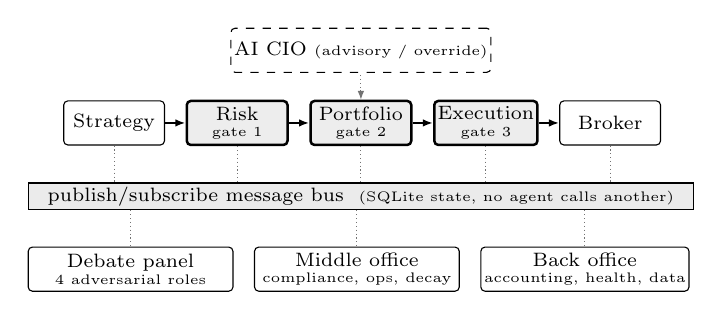
\begin{tikzpicture}[
  font=\scriptsize, node distance=2.6mm,
  ag/.style={draw, rounded corners=1.5pt, minimum height=5.6mm,
             minimum width=1.28cm, align=center, inner sep=1.2pt},
  gate/.style={ag, line width=0.9pt, fill=black!7},
  fl/.style={-{Latex[length=1.3mm]}, thick},
  tap/.style={densely dotted, black!55},
]
\node[ag] (st) {Strategy};
\node[gate, right=of st] (rk) {Risk\\[-2pt]{\tiny gate 1}};
\node[gate, right=of rk] (pf) {Portfolio\\[-2pt]{\tiny gate 2}};
\node[gate, right=of pf] (ex) {Execution\\[-2pt]{\tiny gate 3}};
\node[ag, right=of ex] (br) {Broker};
\foreach \a/\b in {st/rk, rk/pf, pf/ex, ex/br} \draw[fl] (\a) -- (\b);

\node[ag, dashed, above=3.4mm of pf, minimum width=2.4cm] (cio)
  {AI CIO {\tiny(advisory / override)}};
\draw[tap, {Latex[length=1.1mm]}-] (pf) -- (cio);

\node[draw, fill=black!8, below=4.6mm of pf, minimum height=3.4mm,
      minimum width=8.45cm, inner sep=1.2pt] (bus)
  {publish/subscribe message bus \ {\tiny(SQLite state, no agent calls another)}};
\foreach \n in {st, rk, pf, ex, br} \draw[tap] (\n) -- (\n |- bus.north);

\node[ag, below=4.6mm of bus.south west, anchor=north west, minimum width=2.6cm]
  (db) {Debate panel\\[-2pt]{\tiny 4 adversarial roles}};
\node[ag, right=of db, minimum width=2.6cm]
  (mo) {Middle office\\[-2pt]{\tiny compliance, ops, decay}};
\node[ag, right=of mo, minimum width=2.6cm]
  (bo) {Back office\\[-2pt]{\tiny accounting, health, data}};
\foreach \n in {db, mo, bo} \draw[tap] (\n |- bus.south) -- (\n);
\end{tikzpicture}
\caption{The firm as an org chart. Solid arrows are the only route from signal
to broker order, each a bus message the receiving stage may terminate; the
three shaded stages are the nested gates. Debate hangs off the bus: the
PortfolioAgent consults it rather than passing through it, so disabling it
leaves the path untouched.}
\label{fig:arch}
\end{figure}

No agent invokes another. Everything travels as a message on a namespaced
publish/subscribe bus with wildcard subscriptions; in local mode that bus is an
in-process queue and all state lands in SQLite, so the entire firm runs on one
laptop with no infrastructure. That decoupling is what makes the gates
enforceable rather than advisory: no edge skips a stage, so every intent passes
messages the risk and debate agents can intercept. Risk applies symbol-agnostic
weight caps (20\% of NAV) and daily-loss limits; the PortfolioAgent sizes
against database-backed cash, never the key-value mirror; execution checks
kill-switch state, cash sufficiency and a naked-short prohibition, then routes
by symbol so no order reaches a venue that does not trade its asset class.

Three modes trade autonomy against oversight: paper trading executes
immediately in simulation; human approval queues orders for an interactive
decision; fully autonomous makes the debate gate binding and, with no provider
reachable, fails closed. The simulator charges commission on every fill and
applies an Almgren--Chriss-style temporary-impact term
\cite{almgren2001optimal}, and realized P\&L is commission-inclusive, which
forces the cash and P\&L ledgers to agree exactly.

The firm also survives its own components failing: a supervisor restarts
crashed agents from missed heartbeats, exercised in a boot-time
database-contention incident that took down four agents and recovered all of
them without operator action, and a sticky kill switch halts trading on a
drawdown breach until a human clears it. 467 automated tests include regression
pins on the mix weights and the cash/P\&L identity.

\section{Strategy Layer}
\label{sec:sleeves}

Signals originate in independent \emph{sleeves}, each a pure function from
historical bars to target weights, blended at fixed proportions; the validated
mix holds three.

The \textbf{research stack} (weight 0.500, weekly) gates the book with a
Gaussian-mixture regime model on index returns \cite{kritzman2012regime}. In
risk-off states capital rotates into an inverse-volatility blend of
long-duration Treasuries and gold; in risk-on states it ranks the point-in-time
S\&P~500 by 12--1 time-series momentum \cite{jegadeesh1993returns} and quality
\cite{asness2019qmj}, holds the top five, and weights them by hierarchical risk
parity \cite{lopezdeprado2016hrp}, preferred to mean-variance optimization,
whose weights here are dominated by covariance estimation error. Each weight is
capped at half-Kelly.

The \textbf{trend filter} (0.333, weekly) applies Faber's 200-day
moving-average rule \cite{faber2007tactical} to the index proxy, long above
trend and in cash below, with a realized-volatility cap. \textbf{Momentum
rank} (0.167, monthly) takes the top three names by cross-sectional 12--1
momentum at equal weight; the live 20\% position cap holds its standalone
drawdown to $-25.4\%$ against $-59.5\%$ uncapped. The StrategyAgent emits a
signal only when a symbol's net target moves by more than 50 basis points,
which is what keeps turnover low. Unvalidated cryptocurrency and
prediction-market sleeves are carved out pro-rata only when explicitly enabled,
leaving the validated equity mix byte-identical while they are off.

\section{The LLM Debate Gate}
\label{sec:debate}

Under full autonomy every sized trade must survive a structured argument among
four adversarial roles: \textsc{strategy} (the bull case), \textsc{risk} (the
bear case), \textsc{sentiment} (news and crowd positioning) and
\textsc{portfolio} (fit against existing exposure). Every debater receives the
same grounded context and reasons only from it, returning free-text
argumentation plus a discrete vote in
$\{\textsc{for},\textsc{against},\textsc{abstain}\}$ and a confidence in
$[0,1]$. Prose is logged for audit but never parsed for intent, so a debater
who argues eloquently and votes \textsc{against} is counted as against. Roles
are distributed round-robin across whichever providers are configured, and
round two reassigns each debater the opposite role with the first round in
context, forcing engagement with the strongest opposing case and reducing
same-model agreement bias \cite{du2023improving}.

Writing $F$ and $A$ for the \textsc{for} and \textsc{against} vote sets across
both rounds and $c_i$ for confidences, approval requires both conditions of
\eqref{eq:consensus}:
\begin{equation}
\label{eq:consensus}
\begin{aligned}
\frac{\sum_{i \in F} c_i}{\sum_{i \in F \cup A} c_i} \;&>\; 0.55,\\[2pt]
\frac{|F|}{|F| + |A|} \;&\geq\; 0.6.
\end{aligned}
\end{equation}
The two lines guard different failures: the confidence-weighted share lets a
strongly held minority block a lukewarm majority, while the head-count share
prevents one very confident debater from carrying the panel alone. Neither
denominator counts abstentions, so abstaining shrinks the panel instead of
siding with anyone. Malformed output degrades to \textsc{abstain}, and with no
provider reachable the debate rejects: under autonomy the system never trades
on an absence of judgment.

\section{Validation Protocol}
\label{sec:method}

Three rules govern every change to the traded mix.

\textbf{Point-in-time universes.} Ranking today's index members backwards
through history silently conditions on survival \cite{shumway1997delisting}.
This project's earliest backtests made that error, and the edge that motivated
the whole effort evaporated once membership was reconstructed as of each date.
It is a headline here because the machinery that exposed it is the deliverable.

\textbf{Leave-one-out attribution.} Every sleeve is pulled from the mix in turn
and the remainder re-evaluated on point-in-time data. A sleeve keeps its weight
only if removing it does damage.

\textbf{Pre-registered holdout gates.} Candidates are chosen on 2018--2024 and
must then satisfy criteria written down \emph{before} evaluation on an unseen
2008--2017 holdout that spans the financial crisis: Sharpe no worse than the
incumbent, drawdown no deeper, comparable CAGR. Failures ship disabled with the
adverse number recorded. No parameter is ever tuned on holdout data.

\section{Performance}
\label{sec:eval}

Every figure below was regenerated from the repository's harnesses on yfinance
daily bars, with one fill model and one risk-free series across all rows. That
series matters: the realized 13-week Treasury bill averaged 0.31\% across
2008--2017 and 2.33\% across 2018--2024, so a fixed hurdle would punish the
calmer strategy rather than be conservative. All ratios use the realized daily
bill rate \cite{sharpe1994}.

Comparing only against a long-only index is a weak test, so
Table~\ref{tab:perf} carries two peers: \textbf{QAI}, which replicates
aggregate hedge-fund returns and, being a fund rather than a self-reported
index, avoids that literature's backfill and survivorship distortions
\cite{fung2000performance}, and \textbf{AOR}, a conventional 60/40 allocation.
Both post-date the holdout start, so the advantage on that window is a lower
bound.

\begin{table*}[!t]
\caption{Performance across both evaluation windows under one harness, one fill
model and one realized risk-free series. Calmar is CAGR over maximum drawdown;
down-capture is the strategy's mean return on days the index fell, as a
percentage of the index's (lower is better). Final value assumes \$100{,}000 at
the window start. $^\dagger$QAI and AOR post-date the holdout start (88\% and
91\% coverage).}
\label{tab:perf}
\centering
\setlength{\tabcolsep}{4pt}
\footnotesize
\begin{tabular}{lcccccccr}
\toprule
Variant & CAGR & Vol. & Sharpe & Sortino & Calmar & MaxDD & Down-cap. & Final \\
\midrule
\multicolumn{9}{l}{\emph{Selection period, PIT 2018--2024}} \\
Production mix & \textbf{15.8\%} & 15.3\% & \textbf{0.89} & \textbf{1.16} & \textbf{0.88} & $\mathbf{-18.0\%}$ & \textbf{63\%} & \textbf{\$278{,}355} \\
Prior mix (w/ breadth) & 14.6\% & 16.0\% & 0.79 & 1.03 & 0.60 & $-24.2\%$ & 72\% & \$259{,}383 \\
SPY buy-and-hold & 13.6\% & 19.5\% & 0.64 & 0.78 & 0.40 & $-33.7\%$ & n/a & \$244{,}206 \\
Hedge-fund industry (QAI) & 2.5\% & 6.4\% & 0.05 & 0.07 & 0.16 & $-14.9\%$ & 28\% & \$118{,}499 \\
60/40 balanced (AOR) & 5.9\% & 11.5\% & 0.36 & 0.45 & 0.26 & $-22.9\%$ & 58\% & \$149{,}254 \\
\midrule
\multicolumn{9}{l}{\emph{Holdout period, PIT 2008--2017 (unseen at selection)}} \\
Candidate (production) & \textbf{13.0\%} & 12.9\% & \textbf{0.99} & \textbf{1.35} & \textbf{0.68} & $\mathbf{-19.1\%}$ & \textbf{47\%} & \textbf{\$340{,}322} \\
Incumbent (w/ breadth) & 13.0\% & 14.8\% & 0.88 & 1.18 & 0.48 & $-26.9\%$ & 67\% & \$337{,}758 \\
SPY buy-and-hold & 8.5\% & 20.3\% & 0.49 & 0.60 & 0.16 & $-51.9\%$ & n/a & \$226{,}948 \\
Hedge-fund industry (QAI)$^\dagger$ & 3.1\% & 6.0\% & 0.51 & 0.63 & 0.41 & $-7.7\%$ & 25\% & \$130{,}768 \\
60/40 balanced (AOR)$^\dagger$ & 10.2\% & 13.6\% & 0.77 & 0.90 & 0.42 & $-24.4\%$ & 61\% & \$242{,}028 \\
\bottomrule
\end{tabular}
\end{table*}

Both windows tell one story: the mix earns more than the index while carrying
materially less risk, and the surplus is made in bad markets rather than good
ones. Over the selection period it compounds at 15.8\% against 13.6\% at
three-quarters of the index's volatility and roughly half its drawdown, on 78\%
average gross exposure. On the holdout the gap widens to 13.0\% against 8.5\%:
\$100{,}000 ends that decade at \$340{,}322 rather than \$226{,}948, with a
$-19.1\%$ worst drawdown where the index lost $-51.9\%$, and 360 trading days
underwater instead of 835.

Down-capture localises the edge: on the holdout the mix absorbed 47\% of the
index's down-day moves, taking under half the damage through the worst equity
market since 1929, which is why Sortino (1.35) exceeds Sharpe (0.99) by so much
\cite{sortino1994downside}. Against the peers the mix leads on return and on
every risk-adjusted measure in both windows; the industry proxy's 25\%
down-capture is genuinely better, but its Calmar of 0.41 is not, because that
protection is paid for in compounding, 3.1\% against 13.0\%.

\subsection{Attribution and the Sleeve That Was Dropped}

Table~\ref{tab:loo} decomposes the ensemble. Under the pre-registered rule,
leave-one-out is decisive and standalone performance is not, so a sleeve whose
removal \emph{raises} mix Sharpe is a drag regardless of how it looks alone.
The breadth-timing sleeve raised it from 0.79 to 0.89. It had carried 40\% of
the weight. It was removed.

The rest is why an ensemble is warranted. The research stack is load-bearing:
taking it out costs 0.17 of Sharpe, more than any other sleeve adds. The trend
filter is the interesting case, worst in the book standalone at $-0.05$ because
it sits in cash most of its life; removing it costs only 0.03, but its solo
drawdown of $-4.0\%$ against the ensemble's $-18.0\%$ is what it is bought for.
Sleeve correlations span 0.40--0.63, which is the diversification being
purchased. A top-10 variant of momentum rank was tested under the same rule,
failed, and was discarded in favour of top-3.

\begin{table}[!tb]
\caption{Per-sleeve attribution, PIT 2018--2024. LOO is the mix re-run without
that sleeve, weights renormalized. Full-mix Sharpe with breadth = 0.79. All
four verdicts are unchanged from the flat-rate computation under which the
drop decision was taken.}
\label{tab:loo}
\centering
\setlength{\tabcolsep}{4pt}
\footnotesize
\begin{tabular}{lcccc}
\toprule
& \multicolumn{2}{c}{Standalone} & \multicolumn{2}{c}{Leave-one-out} \\
Sleeve & Sharpe & MaxDD & Sharpe & Verdict \\
\midrule
Breadth-timing & 0.44 & $-35.2\%$ & \textbf{0.89} & drags (dropped) \\
Research stack & 0.72 & $-16.4\%$ & 0.63 & carries \\
Trend filter & $-0.05$ & $-4.0\%$ & 0.76 & neutral/hedge \\
Momentum rank & 0.70 & $-25.4\%$ & 0.74 & carries \\
\bottomrule
\end{tabular}
\end{table}

\subsection{Holdout Gate and Multiple Testing}
\label{sec:dsr}

The holdout rows double as an acceptance test. Two thresholds were fixed before
the candidate saw 2008--2017: G1, Sharpe strictly above the incumbent's; G2,
drawdown no more than five points deeper. Both passed with room, 0.99 against
0.88 and a drawdown 7.8 points \emph{shallower}, and the candidate reached the
incumbent's 13.0\% CAGR on lower volatility (12.9\% against 14.8\%) and lower
gross exposure (75\% against 94\%).

A Sharpe ratio chosen as the best of several attempts is biased upward, so the
estimates are deflated. The probabilistic Sharpe ratio gives the chance that
the \emph{true} Sharpe clears a benchmark after correcting for skew and excess
kurtosis \cite{bailey2012psr}; the deflated Sharpe ratio additionally discounts
for picking the best of $N$ trials \cite{bailey2014deflated,harvey2016cross}.
Rather than assume a flattering trial count, deflation uses the twelve Sharpe
ratios this project actually generated, spread $-0.72$ to $0.77$ with variance
$0.159$; a wide spread deflates harder than a generic assumption would.

The edge survives on both windows, more comfortably on the one that counts. On
the selection window (1{,}760 days, SR 0.89) the probability of a positive true
Sharpe is 0.990, of beating the index 0.742, and after deflating for the twelve
trials 0.719; on the holdout (2{,}517 days, SR 0.99) the same three figures are
0.999, 0.941 and 0.846. The inference stops there: 0.742 is evidence, not
proof, and is exactly the number an undeflated Sharpe would have concealed.

\subsection{An Adverse Result and a Live Failure}
\label{sec:polymarket}

Prediction-market prices enter the system as first-class symbols with real
execution support, on the hypothesis that event probabilities drift as informed
flow arrives ahead of resolution. A 7-day probability-momentum sleeve built to
harvest that drift, replayed over CLOB history for the highest-volume markets,
\emph{lost} money: $-8.1\%$ aggregate return, Sharpe $-0.18$, drawdown
$-22.8\%$, hit rate 43.3\%. It ships disabled. A methodology that only ever
approves is not a methodology.

The pipeline has also run live against the Alpaca paper API, sleeve signals
becoming real orders polled to terminal fills. That launch exposed an
underreported failure mode: the local ledger was seeded at \$1M while the
brokerage account held \$100k of paper equity, so sizing against local NAV
produced $3.5\times$ accidental margin exposure. The remedy is a startup
reconciliation guard comparing broker equity against local NAV on connect,
which on a mismatch above 2\% alerts and falls back to simulated execution
rather than trading a ledger it cannot trust. Any architecture whose internal
state can drift from broker truth needs the equivalent.

\section{Isolating the Debate Gate}
\label{sec:aitest}

Everything above measures the rule-based layer, and says nothing about the
marginal value of the LLM panel, which is what this section tests.

\textbf{Design.} Two arms consume an identical signal stream under an identical
fill model. Arm~A disables the gate, so every risk-approved signal executes.
Arm~B makes it binding, so a signal executes only on an \textsc{approved}
conclusion, and a rejected signal leaves that symbol at its previous target,
meaning the gate vetoes exits as well as entries. Sizing, limits and execution
are shared, so any divergence is the gate's, and sleeve targets are a pure
function of bars and date, so both arms consume a byte-identical stream even
after their portfolios separate.

\textbf{Replay, not forward test.} The pre-registered metrics need hundreds of
trades; live paper trading produces a handful per week. The experiment replays
the production mix over 2018--2024 through the real debate engine, and as a
validity check fixed in advance arm~A had to reproduce the published mix within
$\pm 0.02$ Sharpe before any model was called; it does, with $-18.0\%$ drawdown
in both.

\textbf{Leakage, measured rather than assumed away.} A model trained on data
after the window may simply recall what a stock did
\cite{glasserman2023lookahead}. The primary arm
therefore blinds the panel: prompts carry no ticker, no date and no price
level, only six scale-free features (momentum percentile, distance from the
200-day average, realized volatility, drawdown from the 52-week high, index
correlation, regime label), which describe thousands of (security, date) pairs
and leave no retrieval key. A secondary unblinded arm restores ticker and date
on the same signals. The live DebateAgent judges only the strongest signals
within a bounded daily budget and releases the rest undebated; arm~B reproduces
that, so the measurement describes the system as deployed.

\textbf{Arm~C, the rate-matched random gate.} A veto that rejects a large share
of trades mechanically cuts exposure and turnover, and in a trending sample
that alone moves Sharpe, so ``arm~B beat arm~A'' would establish only that the
system traded \emph{less}, not that the panel chose \emph{well}. Arm~C holds
arm~B's measured rejection rate while accepting at random; twenty-five such
gates form a null distribution arm~B must clear to count as judgment.

\textbf{Acceptance criterion, fixed in advance.} The gate stays in the
autonomous pipeline if arm~B's risk-adjusted return is at least arm~A's
\emph{and} the counterfactual P\&L of rejected trades is non-positive.
Otherwise it reverts to advisory-only.

\subsection{Results}
\label{sec:abresults}

The panel concluded 288 debates over 2{,}304 model calls, approving 118 and
rejecting 170: a 59.6\% rejection rate at a median 4.6~seconds per decision. Of
these, 270 enter arm~B, covering 58\% of traded weight, strongest signals
first, which is how the live cost gate allocates its budget; the rest traded
undebated. It was not a rubber stamp: seventy percent of debates split
\textsc{for} against \textsc{against}, and the
\textsc{strategy} debater, briefed to argue the bull case, voted against four
times as often as for (445 to 106) while \textsc{portfolio} and \textsc{risk}
sat near balance.

Binding it made the portfolio worse. Table~\ref{tab:abtest} shows Sharpe
falling from 0.89 to 0.81, Sortino from 1.16 to 1.05, and drawdown deepening
from $-18.0\%$ to $-25.7\%$ on identical signals and fills. CAGR was unchanged
and the arms finished within \$1{,}200 of each other, so the damage is in the
path rather than the destination. The visible change is turnover, collapsing
from 12.72$\times$ to 2.69$\times$ NAV per year: rejecting three signals in
five leaves the book holding positions the sleeves had already decided to trim,
and gross exposure rose from 78\% to 99.8\%. The gate did not select trades so
much as freeze the portfolio.

\begin{table}[!tb]
\caption{Debate-gate A/B, blinded panel, PIT 2018--2024, identical signal
stream and fill model. Arm~C holds arm~B's rejection rate but chooses at random
(25 trials, mean $\pm$ s.d.). $^\ddagger$A sum of independent one-at-a-time
effects, not a realizable P\&L.}
\label{tab:abtest}
\centering
\setlength{\tabcolsep}{4pt}
\footnotesize
\begin{tabular}{lccc}
\toprule
Metric & A (no gate) & B (gate on) & C (random) \\
\midrule
Trades executed & 1{,}867 & 1{,}510 & 1{,}722 \\
Rejection rate & n/a & 59.6\% & 59.6\% \\
Counterfactual P\&L$^\ddagger$ & n/a & $-101\%$ & n/a \\
CAGR & 15.9\% & 15.9\% & n/a \\
Volatility & 15.3\% & 17.3\% & n/a \\
Sharpe ratio & \textbf{0.89} & 0.81 & 0.93 $\pm$ 0.14 \\
Sortino ratio & \textbf{1.16} & 1.05 & n/a \\
Max drawdown & $\mathbf{-18.0\%}$ & $-25.7\%$ & n/a \\
Turnover ($\times$ NAV/yr) & 12.72 & 2.69 & n/a \\
\bottomrule
\end{tabular}
\end{table}

\textbf{The control that settles it.} Arm~C rejects at the same 59.6\% but
picks at random. Twenty-five such gates returned a Sharpe of 0.93 $\pm$ 0.14,
with a 5th--95th percentile band of 0.73--1.19, and the LLM panel beat only 5
of them, an empirical $p$ of 0.80. Fig.~\ref{fig:gate} shows why this
comparison rather than A-versus-B decides the question: the gated curve enters
that band immediately, stays inside it for seven years and ends inside it, so
at no point does deliberate selection separate from arbitrary rejection at the
same rate. Random rejection was in fact better on both mean and median. The
gate's contribution here is the contribution of trading less; without this
control the turnover reduction would have been written up as a risk-management
benefit.

\begin{figure}[!tb]
\centering
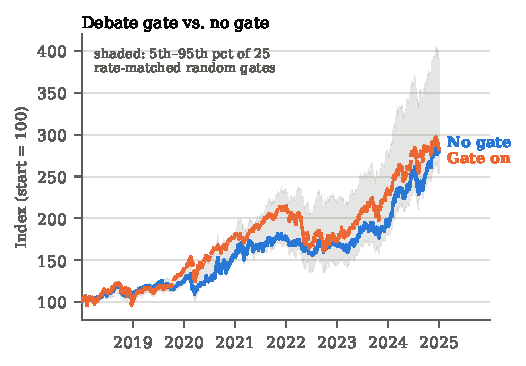
\includegraphics[width=0.95\columnwidth]{fig_gate.pdf}
\caption{The debate-gate experiment. Both arms consume an identical signal
stream; the gated arm executes only what the panel approved. The shaded band is
the 5th--95th percentile of 25 gates rejecting at the same rate but choosing at
random, and the gated arm stays inside it throughout.}
\label{fig:gate}
\end{figure}

\textbf{Was it just remembering?} On the 44 signals judged both ways, the
unblinded panel approved 34.1\% against the blinded panel's 38.6\% and reached
the same verdict on 72.7\% of trades. Revealing ticker and date barely moved
anything, which is what the blinded design needs: the panel worked from its
features rather than recalling outcomes. The paired sample is small.

\textbf{The counterfactual.} Summed over the 161 rejections with price
coverage, the blocked trades would have returned $-101\%$ of NAV, and only 38\%
would have made money. Read naively that says the vetoes were good, which sits
awkwardly beside an arm that performed worse. The two do not conflict: the
counterfactual adds up each blocked weight change against its own forward
return as an independent one-at-a-time event, while the arm those rejections
belong to compounds, overlaps and carries the cost of the stale positions the
vetoes left standing. Where the two disagree the arm-level result and arm~C
carry the weight.

Under the criterion of Sec.~\ref{sec:aitest}, the gate \textbf{fails} the first
condition and reverts to advisory-only. The debate layer keeps its other job:
every trade still carries a recorded argument for why it was permitted, which
has value in a system trading without a human in the loop. It has not earned
authority over execution.

\subsection{What This Says About the Architecture}

Two claims are easy to conflate. The gate did not improve returns; the
\emph{system} was indifferent to that, because the gate occupies a veto slot
where its failure mode is a trade that does not happen. Arm~B's worst outcome
across seven years was 0.08 of Sharpe, not a breached limit or an unbounded
position. That is the property the three-gate structure exists for: a design in
which the least predictable component is load-bearing converts model failure
directly into capital loss \cite{sculley2015debt}. Here it is advisory by
construction, so the consequence is a deployment posture: the gate ships
enabled in its advisory role, where it generates the audit trail, and disabled
as a binding veto until it clears arm~C with more than one model family and a
sentiment role that has a point-in-time news archive.

\section{Limitations}
\label{sec:limits}

\textbf{No real capital.} Everything here is a daily-bar backtest plus a live
\emph{paper}-trading deployment. \textbf{Peers.} QAI and AOR are realized,
net-of-fee streams; the strategy rows charge commission and impact but no fees
and assume unbounded capacity.
\textbf{Residual survivorship bias.} Free daily data omits many delisted
securities \cite{shumway1997delisting}: 85\% of the point-in-time union was
recovered on 2018--2024 and 71\% on 2008--2017, which leaves absolute levels
optimistic, though every arm is affected identically and the ordering holds.
\textbf{One historical path.} A Sharpe from a single realization overstates
certainty \cite{lo2002statistics,bailey2014deflated}; deflation narrows that
without removing it.

\textbf{The gate experiment.} Being a replay, blinding bounds leakage rather
than eliminating it: an extreme feature combination can still narrow the era.
The panel ran on a \emph{single} provider, so cross-family diversity is
implemented but not demonstrated; the \textsc{sentiment} role abstains
structurally for want of a point-in-time news archive, so one voice in four
contributes little; and gating the full stream, rather than the deployed
budgeted subset, is unmeasured. \textbf{Training-corpus priors.} LLM judgments
inherit biases that cannot be audited for a closed model; the
blinded/unblinded agreement rules out one specific failure, not whether those
priors suit the period judged.

\section{Conclusion}

Horizon Capital runs. A firm of decoupled agents with three nested gates
between a signal and a broker order, operating on a laptop against a real
brokerage API, produces a book that would have turned \$100{,}000 into
\$340{,}322 across the financial crisis while the index reached \$226{,}948.
The part worth defending is not the return but the protocol that decided what
was allowed to stay in the system, because that protocol removed more than it
added: the edge that started the project, once point-in-time membership
revealed it as survivorship bias; a breadth sleeve holding 40\% of the mix; a
top-10 momentum variant; and a prediction-market sleeve. What survived returns
Sharpe 0.89 and 0.99 against the index's 0.64 and 0.49 at roughly half the
drawdown, with deflated probabilities of positive true Sharpe of 0.719 and
0.846.

The same protocol then removed the component the project had been most
confident about: under blinded prompts and a control rejecting at the same rate
but choosing at random, the debate gate failed to beat the control, and the
improvement that would otherwise have been claimed was a fivefold turnover
reduction wearing a different hat. That control belongs in any study of an LLM
gate, filter or veto, because such mechanisms move performance by themselves.
None of this shows that language models cannot contribute to a trading system;
it shows that this gate, on these signals, did not, and that the only reason
anyone knows is that it was checked. Next steps: multiple model families, a
point-in-time news archive for the sentiment role, and the full signal stream.

\begin{thebibliography}{20}
\setlength{\itemsep}{0pt plus 0.3pt}

\bibitem{liu2020finrl}
X.-Y.~Liu, H.~Yang, Q.~Chen, R.~Zhang, L.~Yang, B.~Xiao, and C.~D.~Wang,
``FinRL: A deep reinforcement learning library for automated stock trading in
quantitative finance,'' \emph{Deep RL Workshop, NeurIPS}, 2020.
\emph{arXiv:2011.09607}.

\bibitem{xiao2024tradingagents}
Y.~Xiao, E.~Sun, D.~Luo, and W.~Wang, ``TradingAgents: Multi-agents LLM
financial trading framework,'' \emph{arXiv:2412.20138}, 2024.

\bibitem{yu2023finmem}
Y.~Yu, H.~Li, Z.~Chen, Y.~Jiang, Y.~Li, D.~Zhang, R.~Liu, J.~W.~Suchow, and
K.~Khashanah, ``FinMem: A performance-enhanced LLM trading agent with layered
memory and character design,'' \emph{arXiv:2311.13743}, 2023.

\bibitem{du2023improving}
Y.~Du, S.~Li, A.~Torralba, J.~B.~Tenenbaum, and I.~Mordatch, ``Improving
factuality and reasoning in language models through multiagent debate,''
\emph{arXiv:2305.14325}, 2023.

\bibitem{glasserman2023lookahead}
P.~Glasserman and C.~Lin, ``Assessing look-ahead bias in stock return
predictions generated by GPT sentiment analysis,'' \emph{arXiv:2309.17322},
2023.

\bibitem{sculley2015debt}
D.~Sculley \emph{et al.}, ``Hidden technical debt in machine learning
systems,'' in \emph{Advances in Neural Information Processing Systems
(NeurIPS)}, 2015.

\bibitem{jegadeesh1993returns}
N.~Jegadeesh and S.~Titman, ``Returns to buying winners and selling losers:
Implications for stock market efficiency,'' \emph{Journal of Finance},
vol.~48, no.~1, pp. 65--91, 1993.

\bibitem{faber2007tactical}
M.~T.~Faber, ``A quantitative approach to tactical asset allocation,''
\emph{Journal of Wealth Management}, vol.~9, no.~4, pp. 69--79, 2007.

\bibitem{asness2019qmj}
C.~S.~Asness, A.~Frazzini, and L.~H.~Pedersen, ``Quality minus junk,''
\emph{Review of Accounting Studies}, vol.~24, pp. 34--112, 2019.

\bibitem{lopezdeprado2016hrp}
M.~L\'opez~de~Prado, ``Building diversified portfolios that outperform
out of sample,'' \emph{Journal of Portfolio Management}, vol.~42, no.~4,
pp. 59--69, 2016.

\bibitem{kritzman2012regime}
M.~Kritzman, S.~Page, and D.~Turkington, ``Regime shifts: Implications for
dynamic strategies,'' \emph{Financial Analysts Journal}, vol.~68, no.~3,
pp. 22--39, 2012.

\bibitem{almgren2001optimal}
R.~Almgren and N.~Chriss, ``Optimal execution of portfolio transactions,''
\emph{Journal of Risk}, vol.~3, no.~2, pp. 5--39, 2001.

\bibitem{bailey2014deflated}
D.~H.~Bailey and M.~L\'opez~de~Prado, ``The deflated Sharpe ratio:
Correcting for selection bias, backtest overfitting and non-normality,''
\emph{Journal of Portfolio Management}, vol.~40, no.~5, pp. 94--107, 2014.

\bibitem{bailey2012psr}
D.~H.~Bailey and M.~L\'opez~de~Prado, ``The Sharpe ratio efficient frontier,''
\emph{Journal of Risk}, vol.~15, no.~2, pp. 3--44, 2012.

\bibitem{harvey2016cross}
C.~R.~Harvey, Y.~Liu, and H.~Zhu, ``$\ldots$ and the cross-section of expected
returns,'' \emph{Review of Financial Studies}, vol.~29, no.~1, pp. 5--68,
2016.

\bibitem{lo2002statistics}
A.~W.~Lo, ``The statistics of Sharpe ratios,'' \emph{Financial Analysts
Journal}, vol.~58, no.~4, pp. 36--52, 2002.

\bibitem{sharpe1994}
W.~F.~Sharpe, ``The Sharpe ratio,'' \emph{Journal of Portfolio Management},
vol.~21, no.~1, pp. 49--58, 1994.

\bibitem{sortino1994downside}
F.~A.~Sortino and L.~N.~Price, ``Performance measurement in a downside risk
framework,'' \emph{Journal of Investing}, vol.~3, no.~3, pp. 59--64, 1994.

\bibitem{shumway1997delisting}
T.~Shumway, ``The delisting bias in CRSP data,'' \emph{Journal of Finance},
vol.~52, no.~1, pp. 327--340, 1997.

\bibitem{fung2000performance}
W.~Fung and D.~A.~Hsieh, ``Performance characteristics of hedge funds and
commodity funds: Natural vs. spurious biases,'' \emph{Journal of Financial and
Quantitative Analysis}, vol.~35, no.~3, pp. 291--307, 2000.

\end{thebibliography}

\end{document}
